\chapter{Contexte physique et état de l'art}\label{chap:introduction}

\vspace{1cm}

\textit{Dans ce premier chapitre introductif, nous allons décrire le contexte physique des milieux granulaires qui a motivé ce travail de recherche, en passant en revue l'état de l'art des différents modèles issus de la mécanique du contact, ainsi que les méthodes de résolution référencées dans la littérature permettant de résoudre les problèmes de contact en dynamique multi-corps.}

\vspace{1cm}

\minitoc

\newpage

\section{Milieux granulaires et modèles de contact}

Les milieux granulaires sont des matériaux se présentant sous formes de grains distincts de taille assez grande (environ $100$ $\mu m$), et qui interagissent lors de collisions. Ce type de milieu est souvent présent dans notre vie de tous les jours (sable, riz, maïs, sucre, flocons de neige, ...), ce qui en fait un champ d'étude relativement récent, et dont la description peut avoir plusieurs approches. Plusieurs domaines d'études s'intéressent à ces systèmes, très présents dans de nombreux phénomènes naturels (dunes de sable, avalanches de neige, ballast, ...), mais également dans plusieurs applications industrielles telles que l'agro-alimentaire, l'industrie pharmaceutique ou encore le bâtiment, et où ils représentent la seconde matière utilisée en termes de quantité après l'eau. Appréhender ces systèmes à caractère divisé ainsi que leurs propriétés devient donc un enjeu majeur aussi bien pour les industriels, confrontés principalement à des problèmes de stockage et de transport, que pour les géophysiciens qui s'intéressent à ces milieux particulièrement complexes et naturellement difficiles à décrire. Ce qui en fait une problématique de recherche particulièrement pertinente car elle pose de nombreux défis à la communauté scientifique. L'omniprésence de ces milieux dans notre quotidien a incité au recours à la simulation numérique, permettant ainsi de s'affranchir de nombreuses phases de tests grandeur nature, longues et onéreuses. La croissance de la puissance de calcul a rendu possible le traitement d'échantillons réalistes et excessivement complexes de façon rapide, au détriment parfois de la fiabilité des résultats numériques obtenus.\\
Par ailleurs, en l'absence d'un cadre général permettant de décrire les propriétés de ces milieux multi-corps et multi-contact, il est nécessaire de considérer certaines hypothèses sur les états physiques des matériaux granulaires pour étudier leurs comportement. Ainsi, les milieux granulaires peuvent présenter des comportements semblables à ceux d'un solide lorsque ceux-ci s'empilent les uns sur les autres pour former un bloc compact, à ceux d'un liquide dans le cadre d'écoulements granulaires, ou encore à ceux d'un gaz lorsque les grains constituant ces milieux sont agités dans tous les sens (voir Figure \ref{solide_liq_gaz}).

\begin{figure}[!h]
        \centering
        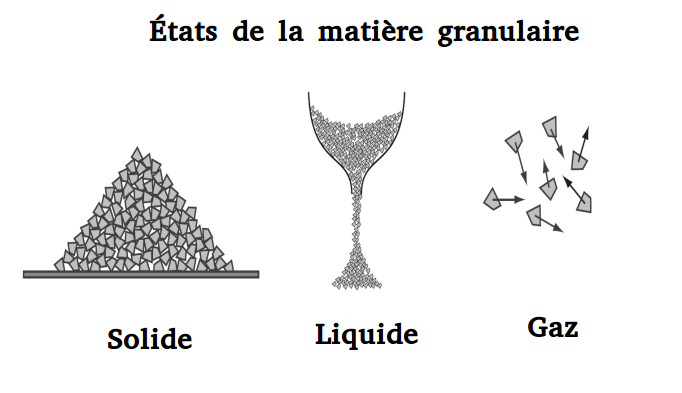
\includegraphics[width=0.55\textwidth]{chapitres/chapitre_0_Introduction/figures/solide_liquide_gaz.png}
        \caption{Représentation des trois états physiques des matériaux granulaires.}
        \label{solide_liq_gaz}    
    \end{figure}

Prédire donc quantitativement un écoulement de tas de sable par exemple, nécessite de bien connaître le modèle étudié, en supposant certaines conditions sur les propriétés mécaniques du milieu et les lois d'interaction de ces systèmes multi-corps. Dans ce sens, plusieurs paramètres physiques et numériques sont à considérer lorsque l'on souhaite simuler numériquement des collections de corps rigides ou déformables, caractérisée par un grand nombre de contacts simultanés.\\

Différentes approches mécaniques permettent de modéliser la dynamique granulaire. Celles-ci sont regroupées sous le terme de \textit{Méthodes des Éléments Discrets} (DEM) dont le développement est initié par les travaux précurseurs de P. A. Cundall [Cundall, \cite{cundall1971measurement}], [Cundall \& Strack, \cite{cundall1979discrete}], qui ont développé la \textit{Méthode des Éléments Distincts} pour des applications liées à la mécanique des roches et à la simulation des matériaux granulaires. Dans ce cadre, on s'intéresse à la fois aux équations du mouvement Eulériennes qui régissent le comportement de chaque grain, décrites par la seconde loi de Newton, et aux efforts de type contact unilatéral et frottement sec qui y sont appliquées, en ayant recours à un processus de régularisation en temps  et en espace. Les non-linéarités dues aux conditions de contact avec frottement sont traitées par la méthode de répulsion-pénalisation et qui consiste à approcher les conditions initiales par des conditions plus simples. L'effort exercé au point de contact lors d'une collision entre deux grains dépend de la contrainte mécanique de non-interpénétrabilité physique, qui tend naturellement à repousser les grains l'un de l'autre. Cette approche régulière reste pour le moins populaire du fait de sa simplicité, de sa faible empreinte mémoire et de son caractère local, qui la rend particulièrement adaptée à des applications industrielles complexes. S'ensuit alors une longue évolution de ces méthodes et un bon nombre de déclinaisons, telle que la méthode \textit{Molecular Dynamics} (MD) \cite{alder1958prigogine,alder1999molecular,alder1960studies} relative aux échelles macroscopiques. La Méthode \textit{Contact Dynamics} (CD) quant à elle, développée par Moreau \cite{jean1992unilaterality, moreau1977application, moreau1988unilateral, moreau1994numerical, moreau1999sweeping} est très vite étendue aux corps déformables par Jean \cite{jean1999non}, et prendra le nom de \textit{Non Smooth Contact Dynamics} (NSCD). Dans le cadre des milieux granulaires denses, généralement sujets au phénomène de frottement, les lois de comportement qui décrivent la dynamique des contacts y sont formulées par des relations de complémentarité non-linéaires et non-régulières à partir de la loi de contact de Signorini en termes de vitesses et d'impulsions, et de la loi de frottement de Coulomb qui relie la force de frottement à la composante tangentielle de la vitesse \cite{desplanques2015amontons}, conduisant à l'approche \textit{Moreau-Jean time-stepping approach} \cite{moreau1994numerical}. Ce schéma numérique est implicite et la propriété de conservation de l'énergie se maintient contrairement à l'approche DEM. Les conditions de contact entre corps rigides sont assurées au moyen d'un solveur itératif de Gauss-Seidel non-linéaire (NLGS), développé par M. Jean et J. J. Moreau \cite{jean1992unilaterality,moreau1994numerical,jean1999non,moreau1999sweeping}, et dont le processus consiste à considérer successivement chaque contact jusqu'à la convergence. Pour plus de détails sur les aspects numériques et certains développements algorithmiques de la NSCD, se référer à \cite{acary2008numerical,dubois2018contact,fortin2005numerical,jean1992unilaterality,jean1999non}. D'autres alternatives au solveur NLGS telles que les solveurs à gradient conjugué ont été proposées dans \cite{renouf2005conjugate}, avec une analyse particulière dans le cadre du calcul parallèle \cite{renouf2004parallel,visseq2013high}.

\section{Méthodes numériques de résolution et logiciels de simulation}

La formulation non-linéaire de l'approche NSCD est coûteuse en temps de calcul par rapport à la DEM, comme le souligne \cite{dubois2018contact}, en particulier pour les matériaux granulaires comprimés, même si la NSCD permet d'envisager des pas de temps plus grand que la DEM, permettant de résoudre plusieurs contacts simultanés. La résolution numérique des conditions de contact avec frottement est ainsi une étape clé dans le processus de simulation numérique. Les temps de calculs relatifs à cette étape varient considérablement selon la méthode numérique choisie pour résoudre ces problèmes. Les techniques habituellement utilisées dans la littérature pour gérer les non-linéarités dues à ces conditions sont basées sur plusieurs types de méthodes parmis lesquelles celle du bi-potentiel \cite{feng2005bi, joli2008uzawa,dumont2013enhanced} ou du quasi-Lagrangien augmenté \cite{de1991new, fortin2005numerical}. L'efficacité de ces méthodes dépend fortement des coefficients de pénalisation \cite{alart1991mixed, fortin2002improved, fortin2005numerical}. Certaines améliorations ont été proposées pour résoudre ce type de problèmes \cite{dumont2013enhanced, joli2008uzawa}, mais elles sont plus coûteuses en temps de calcul.\\

Récemment, les méthodes type Primal-Dual Active Set (PDAS) sont apparues comme des méthodes prometteuses et pertinentes dans la résolution des problèmes de contact avec frottement en milieu déformable \cite{hintermuller2002primal,hueber2008primal,hueber2005primal}, et ce, en raison de leur efficacité et de leur simplicité de mise en œuvre. Dans cette perspective, l'article intitulé \textit{"Inexact primal–dual active set method for solving elastodynamic frictional contact problems"} \cite{abide2021inexact} a été l'occasion pour nous d'analyser ces méthodes type PDAS sur des problèmes continus de contact unilatéral sans frottement, bilatéral avec frottement de Tresca et unilatéral avec frottement de Coulomb en petites et grandes déformations. Celles-ci sont basées sur le principe suivant: les conditions de contact et de frottement sont reformulées en termes de fonctions de complémentarités non-linéaires dont la solution est fournie directement par la méthode itérative semi-régulière de Newton \cite{hintermuller2002primal, hintermuller2003semismooth}, en d'autres termes, les conditions de contact avec frottement peuvent être formulées en un problème de point fixe lié à un problème de quasi-optimisation. Cependant, il existe très peu de travaux qui se sont intéressés à la résolution numérique des problèmes de contacts en dynamique multi-corps par PDAS. Dans la littérature, il existe peu de références sur les méthodes PDAS pour résoudre les problèmes de contact multi-corps rigides. Sur la base d'une hypothèse de corps pseudo-rigides, Koziara et Bicanic \cite{koziara2008semismooth} ont modifié une technique de Newton semi-régulière pour traiter efficacement le problème de contact et de frottement. Dans le cadre de l'optimisation, Sharaf et Mohammad \cite{sharaf2016active} proposent une méthode type Active Set pour la résolution de Problèmes Linéaires Complémentaires (LCP) définis positifs et semi-définis positifs, dont l'efficacité a été testée uniquement sur le problème des sphères rigides verticales statiques en contacts sans frottement. L'utilisation des méthodes type PDAS pour des systèmes multi-corps rigides débutera réellement par les travaux de Barboteu et Dumont \cite{barboteu2018primal}, qui ont développé une méthode type PDAS pour le traitement local des conditions de contact sans frottement dans le cadre de la NSCD, en mettant en évidence l'efficacité de la méthode à travers une série de comparaisons avec les méthodes du bi-potentiel et du quasi-Lagrangien augmenté sur des cas-tests académiques. D'ailleurs, les études menées dans \cite{barboteu2018primal} sur l'efficacité de la méthode type PDAS ont fait l'objet d'une extension aux systèmes dynamiques multi-corps impliquant du frottement dans le cadre de cette thèse, et ce dans une publication acceptée intitulée \textit{"A Semi-Smooth Newton and Primal-Dual Active Set Method for Non-Smooth Contact Dynamics"} \cite{abide2021semismooth}, et tout récemment, dans une seconde publication soumise \textit{"Unified Primal-Dual Active Set Method for dynamic frictional contact problems"} \cite{abide2021unified}, avec entre autres quelques expériences numériques aussi bien sur des problèmes hyper-élastiques que sur des problèmes impliquant des matériaux granulaires rigides.\\

En ce qui concerne la simulation numérique discrète, plusieurs solveurs ont été développé pour modéliser les interactions entre corps rigides ou déformables lors d'écoulements granulaires. On peut citer notamment YADE-OPEN DEM, offre un framework open source extensible pour les modèles numériques discrets, axé sur la DEM (\cite{vsmilauer2010yade, kozicki2009yade}), ou encore le simulateur LIGGGHTS\cite{goniva2010open}, largement utilisé dans le domaine de la dynamique moléculaire. Si la plupart de ces solveurs sont axés sur la DEM, le Laboratoire de Mécanique et Génie Civile (LMGC) s'est doté d'une plateforme de calcul et de développement \textit{LMGC90} \cite{dubois2013lmgc90} adaptée au cadre NSCD pour les milieux granulaires, et qui s'appuie sur le formalisme mathématique de Moreau et Jean. Elle a connu depuis sa création par M. Jean, de nombreux développements, et a été utilisé comme outil numérique dans de nombreux travaux. On peut citer par exemple les travaux G. Saussine \cite{saussine2004contribution} sur le développement d'une code 3D pour coprs polyédriques, ou encore les travaux de Dbouk, Perales \textit{et al.} \cite{dbouk2016df} sur la plateforme numérique Xper, qui repose sur le couplage du code LMGC90 avec une bibliothèque pour le traitement des écoulements fluides-particules, et sur laquelle nous reviendrons en détail un peu plus tard.\\
Pour nos recherches, nous avons choisi d'implémenter le formalisme numérique NSCD-PDAS dans le logiciel open source MFiX-EXA \cite{garg2012documentation}, qui offre d'une part la possibilité d'hériter du parallélisme, et permet d'autre part de traiter des écoulements granulaires dans un cadre applicatif type industriel. De plus, l'approche DEM implémentée dans le logiciel nous permet d'envisager des comparaisons afin d'évaluer la pertinence de l'approche NSCD dans un contexte de calcul parallèle.

\section{Objectifs de la thèse et plan du manuscrit}

Le propos de cette thèse vise donc à fournir en premier lieu une généralisation de l'approche non-régulière NSCD-PDAS aussi bien pour les problèmes de contacts élastiques et hyper-élastiques que pour ceux en dynamique multi-corps rigide et ce, en complétant les travaux de Barboteu et Dumont dans \cite{barboteu2018primal} avec une extension du frottement dans la méthode semi-régulière de Newton, dont la formulation mathématique complexe nécessite de trouver dans un premier temps les fonctions de complémentarité non-linéaires, puis de les dériver afin de déterminer les points fixes correspondants à cette méthode. En second lieu, des études paramétriques seront menées afin d'évaluer les performances, l'efficacité et la validité des méthodes type PDAS dans le cadre de la NSCD en réalisant des comparaisons en termes de temps CPU, d'itérations et de conservation d'énergie avec d'autres méthodes numériques telles que le bi-potentiel ou le quasi-Lagrangien Augmenté. En dernier lieu, nous envisagerons  plusieurs comparaisons applicatives pertinentes aussi bien académiques que concrètes (tambour, lit fluidisé) entre l'approche NSCD-PDAS et l'approche DEM-CUNDALL dans l'environnement MFiX-EXA, tout en palliant aux nombreux  défis qui se posent en termes de modélisation et de temps de calcul, en ayant recours au paradigme de parallélisation proposé.\\

Pour cela, la partie du manuscrit relative aux contributions apportées durant cette thèse se compose de 3 chapitres. Le premier chapitre introduit le formalisme numérique Active Set sur une série de problèmes classiques issus de la mécanique du contact en milieu déformable. Des résultats numériques sont également présentés dans le cas statique et dynamique.\\
Dans le second chapitre, après avoir décrit les lois de contact et de frottement dans le cadre non-régulier de la NSCD, le traitement numérique des conditions de contact avec frottement par Active Set est détaillé. Une batterie de cas-test est également envisagée à des fins de vérification et de validation de l'approche NSCD-PDAS. Des comparaisons numériques avec d'autres méthodes de résolution seront également présentées.\\
L'implémentation de l'approche NSCD-PDAS dans un solveur granulaire conçu pour fonctionner sur des architectures de calcul intensif est proposée dans le dernier chapitre afin de l'étendre dans un contexte applicatif proche de l'industrie. Des comparaisons avec des benchmarks de références sont réalisés sur des configurations complexes pour en évaluer les performances. 